\section{Introducción}

% Parte de Ainhoa
La demencia se define como un síndrome caracterizado por un deterioro cognitivo que produce alteraciones en la memoria, el pensamiento y el comportamiento de una persona. Esto dificulta la capacidad del paciente para realizar sus actividades sociales o laborales. \cite{Formiga2009} Se estima que hay alrededor de 44 millones de personas con demencia, se prevé que esta cifra será más del triple para 2050. \cite{Long2023}.
La \textit{Enfermedad de Alzheimer} (AD), es la enfermedad más común donde se presenta este síndrome (45-55\%), seguida de la demencia vascular y la demencia por cuerpos de Lewy. La demencia frontotemporal no supera el 5\% en las frecuencias relativas. \cite{GOODMAN201728, GarreOlmo2016}. En este proyecto se estudiará un fenotipo concreto presente en varios casos de demencia, la denominada \textit{Demencia Frontotemporal} (FTD).

% Parte de Mario
La FTD es un fenotipo clínico caracterizado por la degeneración progresiva de funciones cognitivas relacionadas con el comportamiento, la personalidad, y el lenguaje, resultado de procesos neurodegenerativos que afectan principalmente a los lóbulos frontal y temporal del cerebro \cite{snowden2002frontotemporal, ratnavalli2002prevalence, piguet2011behavioural}. Es una de las principales causas de demencia en personas menores de 65 años, presentándose con mayor frecuencia entre los 45 y 65 años \cite{snowden2002frontotemporal,  ratnavalli2002prevalence}. Las variantes clínicas más comunes de la FTD son la variante conductual (bvFTD), experimentada por el 70\% de los pacientes y que afecta la regulación del comportamiento y las emociones \cite{snowden2002frontotemporal, piguet2011behavioural}, y la afasia progresiva primaria (PPA), que afecta las habilidades del lenguaje y se subdivide en variantes no fluente/agramática (nfvPPA), semántica (svPPA) y logopénica (lvPPA) \cite{gorno2011classification}.

% Parte de Carmen
La FTD, al tratarse de un conjunto heterogéneo de fenotipos, muestra conexiones significativas con otras enfermedades neurodegenerativas. En estudios de coocurrencia de términos, \textit{Esclerosis Lateral Amiotrófica} (ELA) y EA son conceptos frecuentemente asociados con FTD, lo que sugiere una relación estrecha \cite{fneur.2024.1399600}. % Sigue parte de Mario
Se puede deducir entonces otras enfermedades neurodegenerativas presentan el fenotipo clínico de la FTD, indicando que hay una neuropatología subyacente que las relaciona, manifestada bajo este conjunto de fenotipos. La degeneración lobar frontotemporal (FTLD) es el término general que agrupa a los fenotipos patológicos que dan lugar al fenotipo clínico de la FTD \cite{neary1998frontotemporal}. La FTLD se clasifica según la acumulación de proteínas anormales en las neuronas. Los subtipos principales incluyen: FTLD-tau, caracterizado por la acumulación de tau hiperfosforilada y asociado fuertemente con la bvFTD \cite{mackenzie2010tau}; FTLD-TDP, que afecta a más del 50\% de los pacientes tau-negativos, estrechamente relacionada con la bvFTD y la svPPA \cite{mackenzie2008atypical}; y FTLD-FUS \cite{mackenzie2010tdp}. % Sigue Carmen 
El ejemplo más sonado en la literatura se relaciona con la ELA, una forma común de enfermedad de la motoneurona (MND) \cite{NHS_MND}, la cual es una enfermedad neurodegenerativa que comparte causas genéticas y neuropatologías con la FTD \cite{10.1093/brain/awr195}. Mutaciones en genes como \textit{C9orf72} \cite{DeJesusHernandez2011}, \textit{TARDBP} \cite{Arai2006} y \textit{OPTN} \cite{Bussi2018} se han identificado en pacientes que presentan el fenotipo FTD, padecen ELA, o con manifestaciones de ambas.  Las expansiones en \textit{C9orf72} una causa frecuente en ambos casos \cite{Balendra2018, DeJesusHernandez2011}. Patológicamente, se han observado disfunciones en el sistema autofagia-lisosoma \cite{Casterton2020} e inclusiones citoplásmicas neuronales tau-negativas pero ubiquitina-positivas \cite{Arai2006} en ambas enfermedades. Pacientes con MND pueden desarrollar afectación cognitiva y evolucionar a FTD \cite{Devenney2015}, e incluso mostrar síntomas típicos de bvFTD \cite{Devenney2019}. Asimismo, el parkinsonismo, especialmente el síndrome corticobasal, presenta solapamientos considerables con la FTD, incluyendo trastornos motores y cognitivos \cite{Orphanet_MND}

% Sigue Mario
En cuanto al diagnóstico, la neuroimagen permite distinguir de manera confiable los subtipos de FTLD de otras demencias, ayudando a correlacionar los síntomas neuropsiquiátricos con los patrones de atrofia cerebral. Técnicas como la Image por Resonancia Magnética (MRI) permiten detectar la atrofia focal en los lóbulos frontal y temporal, típicamente observada en pacientes con bvFTD \cite{gorno2011classification}. Las técnicas de neuroimagen funcional, como la tomografía por emisión de positrones (FDG-PET) y la tomografía por emisión de fotón único (SPECT), se utilizan para identificar áreas de hipometabolismo cerebral, dado que bvFTD muestra hipometabolismo en las regiones frontales \cite{varma2002spect, kanda2008fdgpet} (Figura \ref{fig:comparacion_imagenes_diagnostico}). Estos métodos también son efectivos para caracterizar las variantes de la PPA. La nfvPPA muestra atrofia en la región fronto-insular, mientras que la svPPA afecta a los lóbulos temporales anteriores \cite{gorno2011classification} (Figura \ref{fig:comparacion_imagenes_diagnostico}). Técnicas avanzadas como la PET con amiloide-\(\beta\), han mostrado ser prometedoras para discriminar entre casos atípicos de AD y FTLD \cite{rowe2007imagingamiloid}. Además, se ha avanzado en la comprensión de las bases genéticas de la FTD, con mutaciones en genes como MAPT, GRN y C9orf72, que están implicadas en aproximadamente el 30-50\% de los casos familiares de FTD \cite{sirkis2019recentgenes}.

% Parte de Gonzalo

Siguiendo en esta línea, en torno al 40\% de los casos en los que se expresa la FTD son familiares, es decir tienen un patrón hereditario \cite{pan2013clinic, sirkis2019recentgenes}. De los genes que más frecuentemente se ven implicados, uno es el MAPT, que está implicado en la producción de la proteína tau, un importante mediador en la polimerización y estabilización de los microtúbulos cerebrales \cite{caillet2015regulation}. Algunas mutaciones en el gen GRN provocan una producción reducida de progranulina, que causa neurodegeneración y se asocia típicamente con bvFTD, aunque también se han reportado casos de PPA \cite{bateman2009granulin}. La causa genética más común de la FTD, viene dada por el gen C9ORF72, el cual sufre normalmente una expansión del hexanucleótido GGGGCC en una región no codificante del cromosoma 9 \cite{mackenzie2014neuropathology}.

Otros genes implicados son el gen TARDBP, del cual se han encontrado mutaciones tanto en pacientes con FTD esporádico como familiar \cite{borroni2010tardbp}; el gen VCP, que interviene en diversos procesos celulares, del cual se han encontrado mutaciones en pacientes con FTD negativos en MAPT, GRN y C9ORF72 \cite{wong2018three}; o el gen CHMP2B, que sufre mutaciones de truncamiento o sin sentido, relacionado con la demencia frontotemporal del cromosoma 3 (FTD-3) \cite{m2011frontotemporal}.

En relación con los factores ambientales que afectan al fenotipo, un estudio sugiere una relación entre el trauma craneoencefálico y la FTD \cite{granadillo2008genetica, rosso2003medical}. Además, no se encontró relación con factores como el tabaco, el alcohol, exposición a químicos, pesticidas o insecticidas \cite{rosso2003medical}. 

% Parte de Ainhoa Pérez

Cabe destacar que la esperanza de vida promedio de un paciente que presenta los fenotipos clínicos de la FTD es de 6 a 8 años, variando entre 3 y 20 años según la gravedad y las mutaciones genéticas presentes \cite{Hodges2003}. Aunque no existen tratamientos aprobados por la FDA, las estrategias terapéuticas actuales se adaptan al fenotipo predominante en cada paciente, combinando intervenciones farmacológicas y no farmacológicas para mejorar la calidad de vida y controlar los síntomas \cite{SpringerLink2023}.

Entre los tratamientos farmacológicos más prometedores destacan las terapias génicas, como PBFT02, que corrige mutaciones en el GRN \cite{PassageBio2023}, y otros medicamentos experimentales dirigidos a pacientes con mutaciones en granulina, como el FRM-0334 \cite{MayoClinic2023}. También se emplean estimulantes del sistema nervioso central y antipsicóticos atípicos para manejar los síntomas conductuales \cite{NINDS2023}. En cuanto a las terapias no farmacológicas, se incluyen intervenciones en el estilo de vida y terapias ocupacionales, del habla y físicas para mejorar la funcionalidad y la comunicación de los pacientes.


\begin{figure}[h]
	\centering
	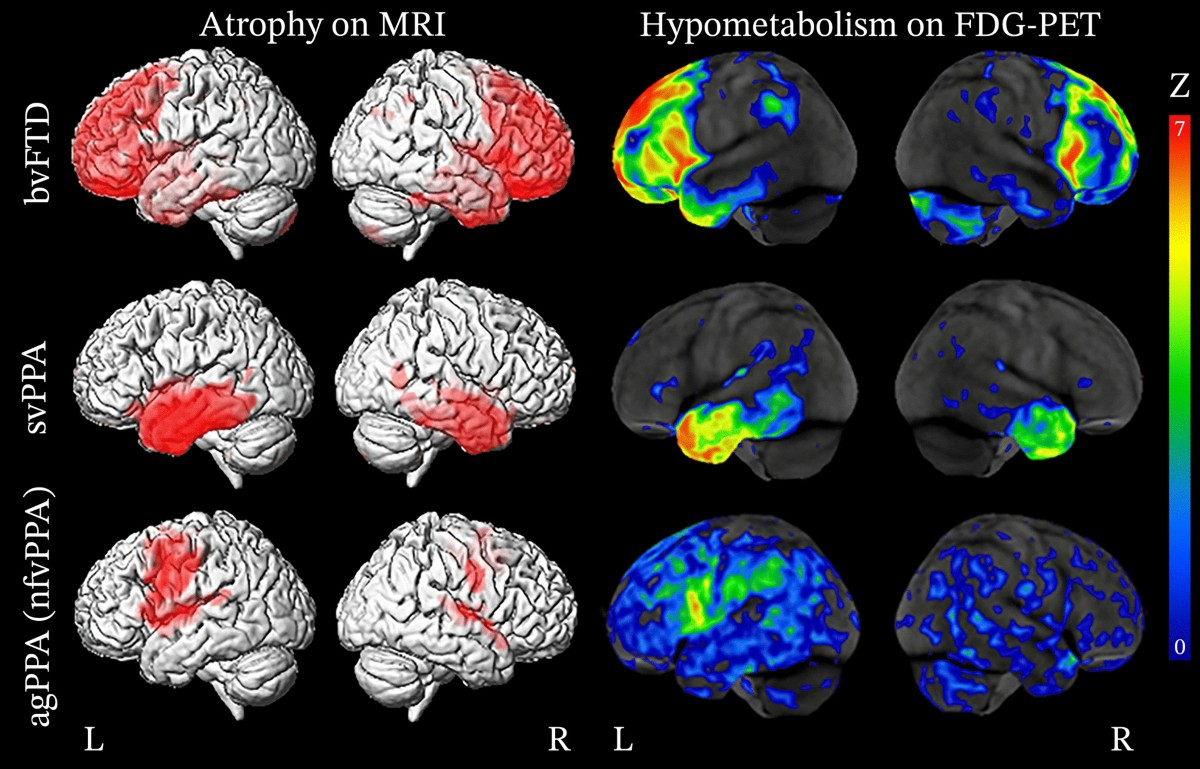
\includegraphics[width=0.75\linewidth]{figures/introduction/differences.jpg}
	\caption{Comparación entre los patrones de atrofia cerebral y el hipometabolismo en diferentes variantes de FTD. En la columna izquierda, reconstrucciones 3D de MRI, que muestran las áreas de atrofia cerebral (en rojo) en tres subtipos de FTD: bvFTD, svPPA, y nfvPPA. En la columna derecha, reconstrucciones 3D de FDG-PET, las cuales indican el hipometabolismo cerebral (en colores) en las mismas regiones afectadas, reflejando la disminución del metabolismo en las áreas afectadas. Los colores cálidos (rojo/amarillo) indican mayor hipometabolismo, mientras que los colores fríos (verde/azul) indican menor hipometabolismo. Imagen tomada de \cite{peet2021neuroimaging}.}
	\label{fig:comparacion_imagenes_diagnostico}
\end{figure}

\section{Objetivos}

Se plantean los siguientes objetivos para este estudio:

\begin{enumerate}
	\item \textbf{RQ1}. ¿Es posible identificar los procesos biológicos implicados en la Demencia Frontotemporal mediante el análisis de la red de interacción proteína-proteína asociado?.
	\item \textbf{RQ2}. ¿Es posible implementar una detección de comunidades sobre la red de interacción proteína-proteína tal que detecte las interacciones clave del fenotipo?
	
	\item \textbf{SRQ1}. Bajo el marco de la biología de sistemas, integrar el conocimiento estadístico de la red, los resultados de la detección de comunidades, y el análisis funcional para cumplir con los objetivos expuestos.
\end{enumerate}

